\documentclass{article}
\usepackage{pgfplots}
\usepackage{amsmath}
\usepackage{amssymb}
\usepackage{tikz,mathpazo}
\usetikzlibrary{calc}
\usetikzlibrary{arrows,shapes}
\usetikzlibrary{shapes.geometric}
\usetikzlibrary{arrows.meta}
\usepackage{graphics,graphicx}
\usetikzlibrary{external}
\tikzexternalize
\tikzset{external/system call={latex \tikzexternalcheckshellescape
  -halt-on-error -interaction=batchmode -jobname "\image" "\texsource";
  dvips -o "\image".eps "\image".dvi}}
  % pdflatex --shell-escape *.tex

\begin{document}

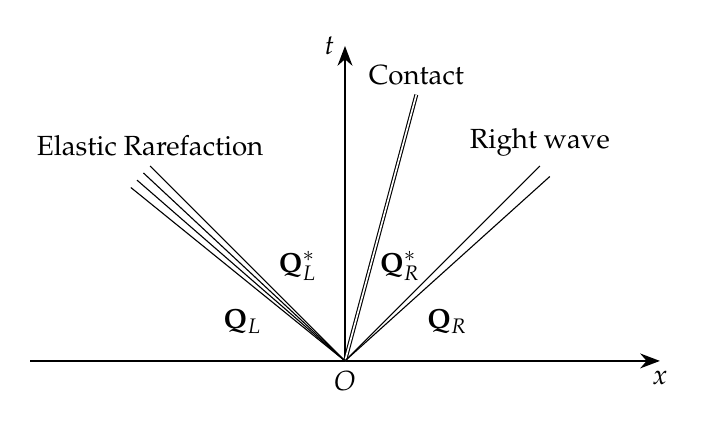
\begin{tikzpicture}
	\draw [line width =1pt,-{Stealth[length=2.5mm]}] (0,0) -- (4,0) node[below]{$x$};
	\draw [line width =1pt] (-4,0) -- (0,0);
	\draw [line width =1pt,-{Stealth[length=2.5mm]}] (0,0) -- (0,4) node[left]{$t$};
	\draw [double](0,0) -- ([turn]165:3.5)   node [above]{Contact};
	\draw  (0,0) node [below]{$O$} -- ([turn]135:3.5) node [above]{Right wave};
	\draw  (0,0) -- ([turn]132:3.5);
	\draw  (0,0) -- ([turn]-135:3.5) node [above]{Elastic Rarefaction};
	\draw  (0,0) -- ([turn]-133:3.5);
	\draw  (0,0) -- ([turn]-131:3.5);
	\draw  (0,0) -- ([turn]-129:3.5);
	\node at (-1.3,0.5) {$\mathbf{Q}_L$};
	\node at (-0.6,1.2) {$\mathbf{Q}_L^*$};
	\node at (0.7,1.2) {$\mathbf{Q}_R^*$};
	\node at (1.3,0.5) {$\mathbf{Q}_R$};
\end{tikzpicture}
%
  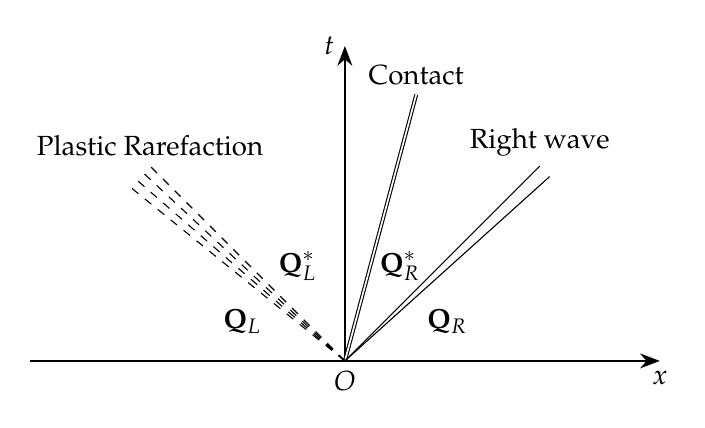
\begin{tikzpicture}
	\draw [line width =1pt,-{Stealth[length=2.5mm]}] (0,0) -- (4,0) node[below]{$x$};
	\draw [line width =1pt] (-4,0) -- (0,0);
	\draw [line width =1pt,-{Stealth[length=2.5mm]}] (0,0) -- (0,4) node[left]{$t$};
	\draw [double](0,0) -- ([turn]165:3.5)   node [above]{Contact};
	\draw  (0,0) node [below]{$O$} -- ([turn]135:3.5) node [above]{Right wave};
	\draw  (0,0) -- ([turn]132:3.5);
	\draw [dashed] (0,0) -- ([turn]-135:3.5) node [above]{Plastic Rarefaction};
	\draw  [dashed](0,0) -- ([turn]-133:3.5);
	\draw  [dashed](0,0) -- ([turn]-131:3.5);
	\draw  [dashed](0,0) -- ([turn]-129:3.5);
	\node at (-1.3,0.5) {$\mathbf{Q}_L$};
	\node at (-0.6,1.2) {$\mathbf{Q}_L^*$};
	\node at (0.7,1.2) {$\mathbf{Q}_R^*$};
	\node at (1.3,0.5) {$\mathbf{Q}_R$};
\end{tikzpicture}


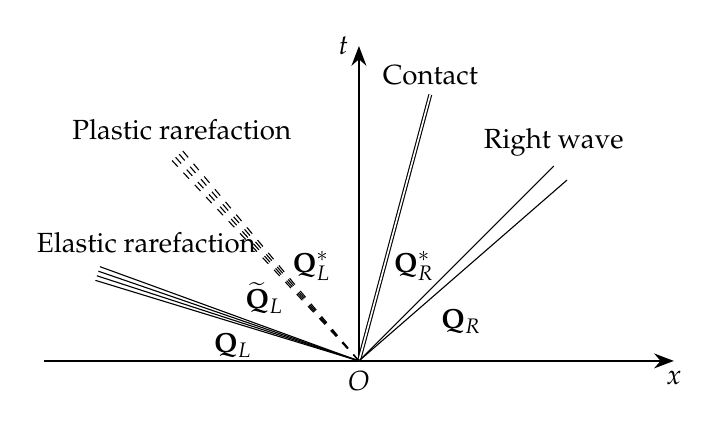
\begin{tikzpicture}
    \draw [line width =1pt,-{Stealth[length=2.5mm]}] (0,0) -- (4,0) node[below]{$x$};
    \draw [line width =1pt] (-4,0) -- (0,0);
    \draw [line width =1pt,-{Stealth[length=2.5mm]}] (0,0) -- (0,4) node[left]{$t$};
    \draw (0,0) node [below]{$O$} -- ([turn]-110:3.5);
    \draw (0,0) -- ([turn]-109:3.5);
    \draw (0,0) -- ([turn]-108:3.5);
	\draw (0,0) -- ([turn]-107:3.5);
    \draw [double](0,0) -- ([turn]165:3.5)   node [above]{Contact};
    \draw  (0,0) -- ([turn]135:3.5) node [above]{Right wave};
    \draw  (0,0) -- ([turn]131:3.5);
    \draw  (0,0)[dashed] -- ([turn]-140:3.5) node [above]{Plastic rarefaction} ;
    \draw  (0,0)[dashed] -- ([turn]-139:3.5) ;
    \draw  (0,0)[dashed] -- ([turn]-138:3.5) ;
    \draw  (0,0)[dashed] -- ([turn]-137:3.5) ;
    \node at (-1.6,0.2) {$\mathbf{Q}_L$};
    \node at (-1.2,0.8) {$\widetilde{\mathbf{Q}}_L$};
    \node at (-0.6,1.2) {$\mathbf{Q}_L^*$};
    \node at (0.7,1.2) {$\mathbf{Q}_R^*$};
    \node at (1.3,0.5) {$\mathbf{Q}_R$};
	\node at (-2.7,1.5) {Elastic rarefaction};
\end{tikzpicture}


  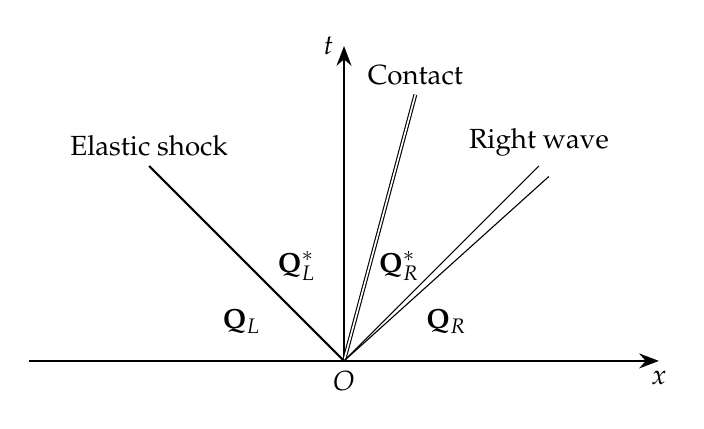
\begin{tikzpicture}
	\draw [line width =1pt,-{Stealth[length=2.5mm]}] (0,0) -- (4,0) node[below]{$x$};
	\draw [line width =1pt] (-4,0) -- (0,0);
	\draw [line width =1pt,-{Stealth[length=2.5mm]}] (0,0) -- (0,4) node[left]{$t$};
	\draw [double](0,0)  -- ([turn]165:3.5)   node [above]{Contact};
	\draw  (0,0) -- ([turn]135:3.5) node [above]{Right wave};
	\draw  (0,0) -- ([turn]132:3.5);
	\draw  (0,0) [line width = 0.8pt] node [below]{ $O$ }  -- ([turn]-135:3.5) node [above]{Elastic shock};
	\node at (-1.3,0.5) {$\mathbf{Q}_L$};
	\node at (-0.6,1.2) {$\mathbf{Q}_L^*$};
	\node at (0.7,1.2) {$\mathbf{Q}_R^*$};
	\node at (1.3,0.5) {$\mathbf{Q}_R$};
\end{tikzpicture}

  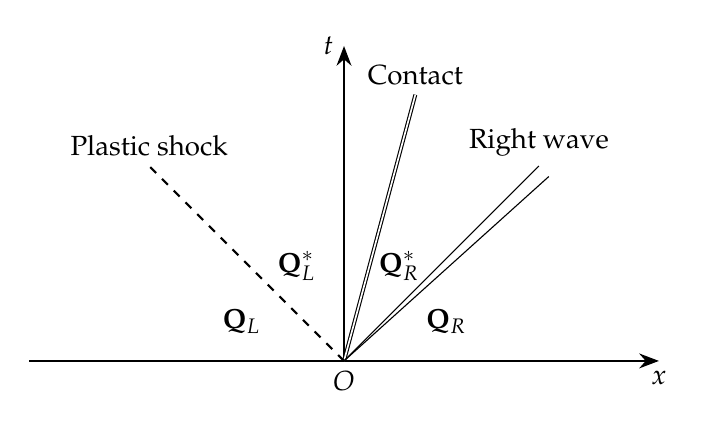
\begin{tikzpicture}
	\draw [line width =1pt,-{Stealth[length=2.5mm]}] (0,0) -- (4,0) node[below]{$x$};
	\draw [line width =1pt] (-4,0) -- (0,0);
	\draw [line width =1pt,-{Stealth[length=2.5mm]}] (0,0) -- (0,4) node[left]{$t$};
	\draw [double](0,0)  -- ([turn]165:3.5)   node [above]{Contact};
	\draw  (0,0) -- ([turn]135:3.5) node [above]{Right wave};
	\draw  (0,0) -- ([turn]132:3.5);
	\draw  (0,0) [dashed, line width = 0.8pt] node [below]{ $O$ }  -- ([turn]-135:3.5) node [above]{Plastic shock};
	\node at (-1.3,0.5) {$\mathbf{Q}_L$};
	\node at (-0.6,1.2) {$\mathbf{Q}_L^*$};
	\node at (0.7,1.2) {$\mathbf{Q}_R^*$};
	\node at (1.3,0.5) {$\mathbf{Q}_R$};
\end{tikzpicture}

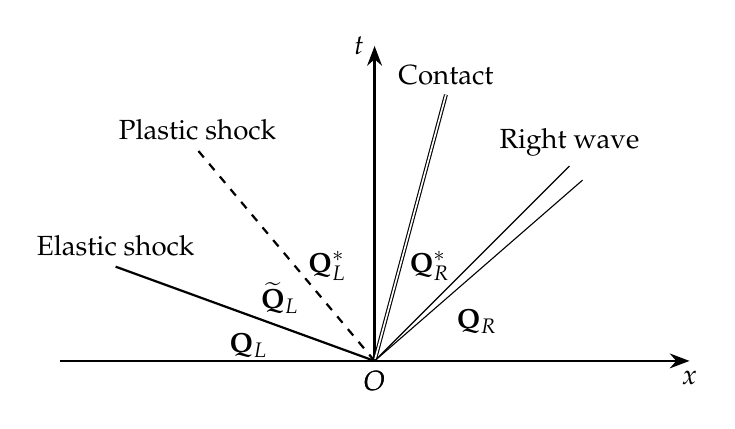
\begin{tikzpicture}
    \draw [line width =1pt,-{Stealth[length=2.5mm]}] (0,0) -- (4,0) node[below]{$x$};
    \draw [line width =1pt] (-4,0) -- (0,0);
    \draw [line width =1pt,-{Stealth[length=2.5mm]}] (0,0) -- (0,4) node[left]{$t$};
	\draw (0,0) [line width =0.8pt] node [below]{$O$} -- ([turn]-110:3.5) node [above]{Elastic shock};
    \draw [double](0,0) -- ([turn]165:3.5)   node [above]{Contact};
	\draw  (0,0) node[below]{$O$} -- ([turn]135:3.5) node [above]{Right wave};
    \draw  (0,0) -- ([turn]131:3.5);
	\draw  (0,0)[dashed, line width =0.8pt] -- ([turn]-140:3.5) node [above]{Plastic shock} ;
    \node at (-1.6,0.2) {$\mathbf{Q}_L$};
    \node at (-1.2,0.8) {$\widetilde{\mathbf{Q}}_L$};
    \node at (-0.6,1.2) {$\mathbf{Q}_L^*$};
    \node at (0.7,1.2) {$\mathbf{Q}_R^*$};
    \node at (1.3,0.5) {$\mathbf{Q}_R$};
\end{tikzpicture}

\tikzstyle{startstop} = [rectangle, rounded corners, minimum width = 2cm, minimum height=1cm,text centered, draw = black, fill = red!30]
\tikzstyle{io} = [trapezium, trapezium left angle=70, trapezium right angle=110, minimum width=2cm, minimum height=1cm, text centered, draw=black, fill = blue!40]
\tikzstyle{process} = [rectangle, minimum width=3cm, minimum height=1cm, text centered, draw=black, fill = yellow!50]
\tikzstyle{decision} = [diamond, aspect = 3, text centered, draw=black, fill = green!30]
% 箭头形式
\tikzstyle{arrow} = [->,>=stealth]

\begin{tikzpicture}[node distance=2cm]
%定义流程图具体形状
\node (start1) [startstop] {$\rho_L^*$};
\node (start2) [startstop,right of=start1, xshift = 1cm] {$\rho_R^*$};
\node (pro1) [process, below of=start1, yshift=0.2cm, left of=start1, xshift=0.8cm] {$p_L^*,s_{xxL}^*,u_L^*$};
\node (pro2) [process, right of=pro1, xshift= 3.7cm] {$p_R^*,s_{xxR}^*,u_R^*$};
\node (dec1) [decision, below of=pro1, yshift= -0.5cm, xshift=3.0cm] {Convergence ?};
\node (stop) [startstop, below of=dec1] {Output with $\mathbf{Q}_L^*$ and $\mathbf{Q}_R^*$};

%连接具体形状
\draw [arrow](start1) -- (pro1);
\draw [arrow](start2) -- (pro2);
\draw [arrow](pro1) -- (dec1);
\draw [arrow](pro2) -- (dec1);
\draw [arrow](dec1) -- ($(dec1.east) + (2.5,0)$) node[anchor=north] {NO}  |- node [anchor =south] {A new $\rho_R^*$} (start2);
\draw [arrow](dec1) -- ($(dec1.west) + (-2.8,0)$) node[anchor=north] {NO} |- node [anchor =south] {A new $\rho_L^*$}(start1);
%\draw [arrow](dec1) -- ($(dec1.east) + (1.5,0)$) node[anchor=north] {NO} |- (pro2);
\draw [arrow](dec1) -- node[anchor=west] {YES} (stop);
\end{tikzpicture}

  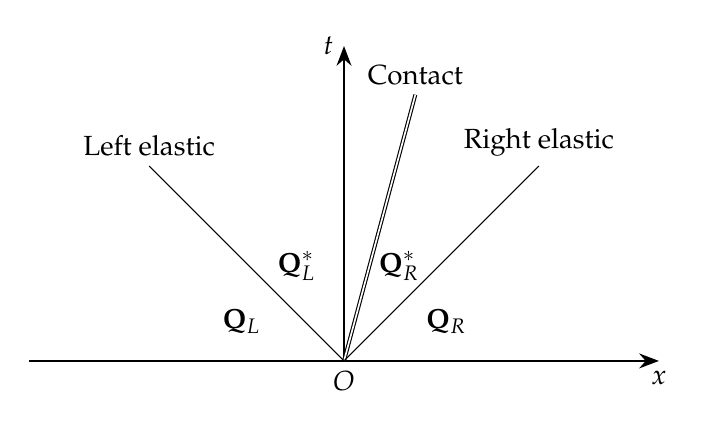
\begin{tikzpicture}
    \draw [line width =1pt,-{Stealth[length=2.5mm]}] (0,0) -- (4,0) node[below]{$x$};
    \draw [line width =1pt] (-4,0) -- (0,0);
    \draw [line width =1pt,-{Stealth[length=2.5mm]}] (0,0) -- (0,4) node[left]{$t$};
    \draw [double](0,0) -- ([turn]165:3.5)   node [above]{Contact};
	\draw  (0,0) node[below]{$O$} -- ([turn]135:3.5) node [above]{Right elastic};
    \draw  (0,0) -- ([turn]-135:3.5) node [above]{Left elastic} ;
    \node at (-1.3,0.5) {$\mathbf{Q}_L$};
    \node at (-0.6,1.2) {$\mathbf{Q}_L^*$};
    \node at (0.7,1.2) {$\mathbf{Q}_R^*$};
    \node at (1.3,0.5) {$\mathbf{Q}_R$};
\end{tikzpicture}

% Half Riemann solver 


  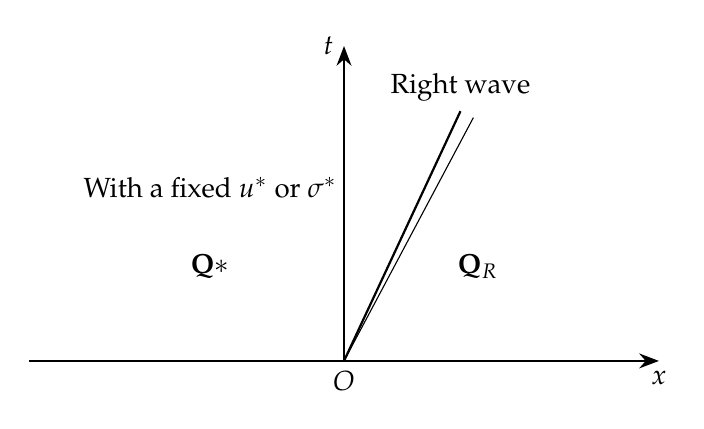
\begin{tikzpicture}
	\draw [line width =1pt,-{Stealth[length=2.5mm]}] (0,0) -- (4,0) node[below]{$x$};
	\draw [line width =1pt] (-4,0) -- (0,0);
	\draw [line width =1pt,-{Stealth[length=2.5mm]}] (0,0) -- (0,4) node[left]{$t$};
%	\draw [double](0,0)  -- ([turn]165:3.5)   node [above]{Contact};

	\draw  (0,0) -- ([turn]152:3.5);
	\draw  (0,0) [line width = 0.8pt] node [below]{ $O$ }  -- ([turn]155:3.5) node [above]{Right wave};
	\node at (-1.7,1.2) {$\mathbf{Q}*$};
	\node at (-1.7,2.2) {With a fixed $u^*$ or $\sigma^*$};
	\node at (1.7,1.2) {$\mathbf{Q}_R$};
\end{tikzpicture}


  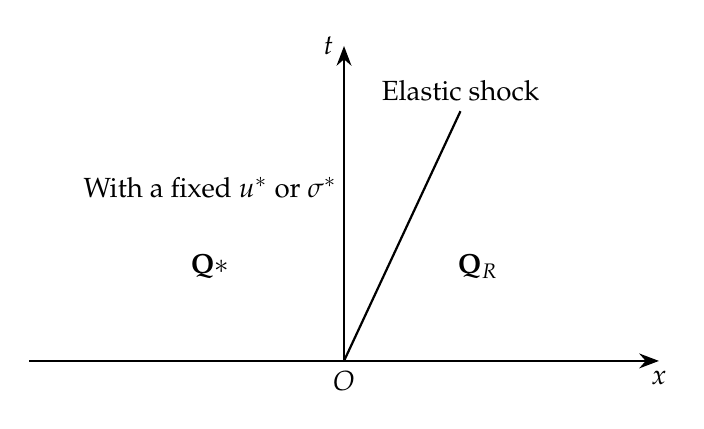
\begin{tikzpicture}
	\draw [line width =1pt,-{Stealth[length=2.5mm]}] (0,0) -- (4,0) node[below]{$x$};
	\draw [line width =1pt] (-4,0) -- (0,0);
	\draw [line width =1pt,-{Stealth[length=2.5mm]}] (0,0) -- (0,4) node[left]{$t$};
%	\draw [double](0,0)  -- ([turn]165:3.5)   node [above]{Contact};

	\draw  (0,0) [line width = 0.8pt] node [below]{ $O$ }  -- ([turn]155:3.5) node [above]{Elastic shock};
	\node at (-1.7,1.2) {$\mathbf{Q}*$};
	\node at (-1.7,2.2) {With a fixed $u^*$ or $\sigma^*$};
	\node at (1.7,1.2) {$\mathbf{Q}_R$};
\end{tikzpicture}

 \end{document}
